\titreTD{\thenumTD}{Mod\`ele ondulatoire}

\begin{center}
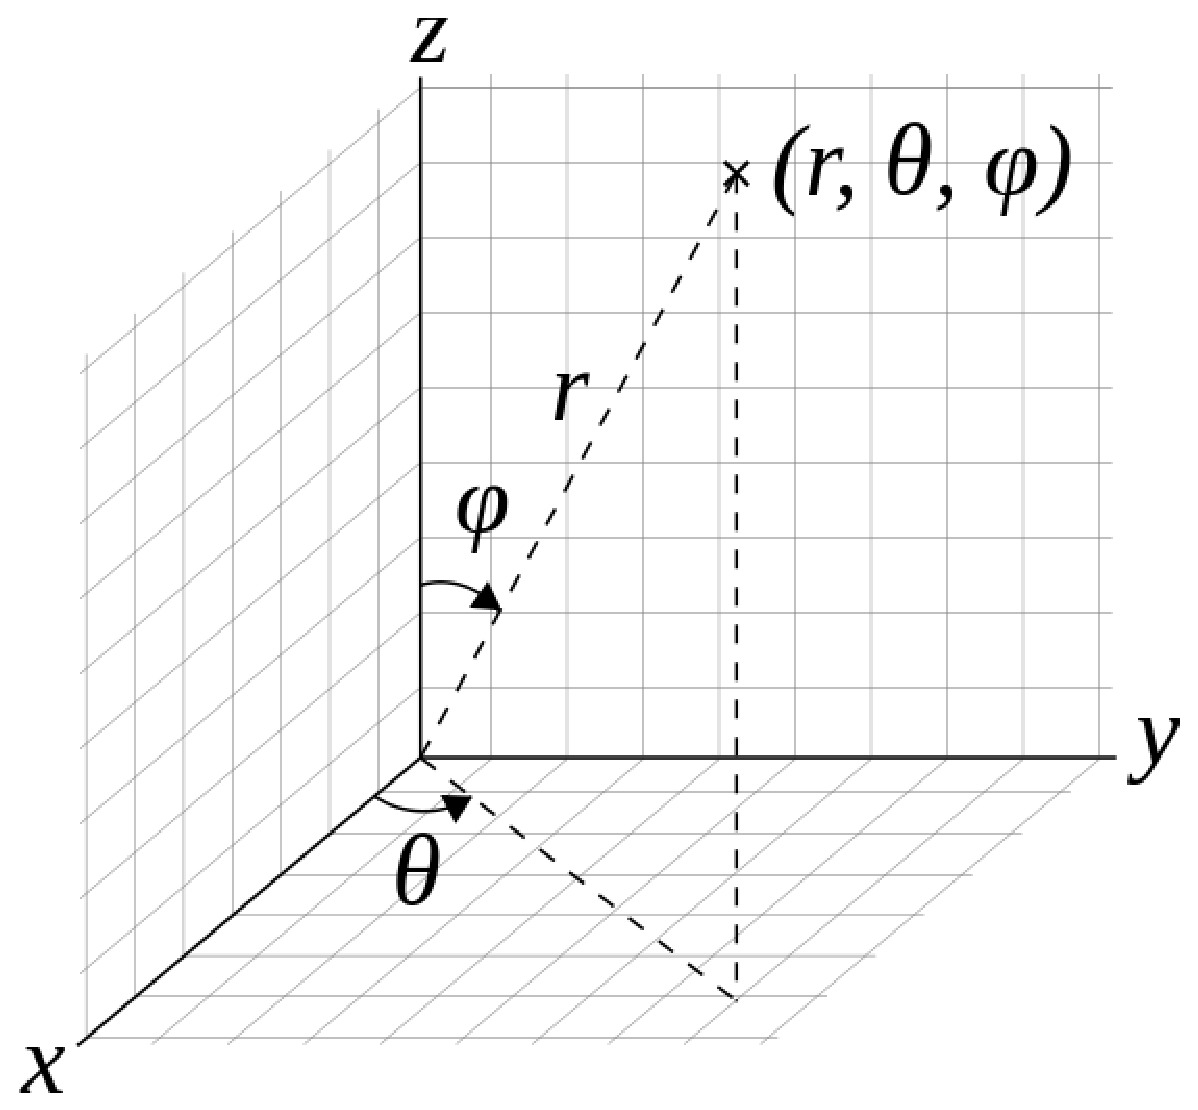
\includegraphics[height=9.5cm]{figure/spheriques.eps}\\
\end{center}

\exo{Fonctions de type ns}

Les trac\'es de la partie radiale des orbitales $1s$, $2s$ et $3s$ de l'atome d'hydrog\`ene 
sont repr\'esent\'es ci-apr\`es.
Tracez de mani\`ere qualitative la densit\'e de probabilit\'e radiale pour les orbitales
$1s$, $2s$ et $3s$. Commentez. 

\clearpage
\begin{center}
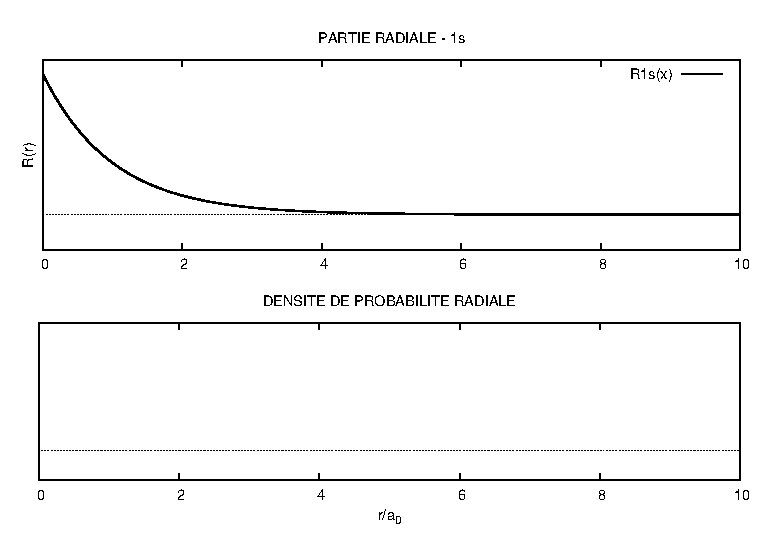
\includegraphics[angle=90,width=\textwidth]{figure/rad1s.eps}
\end{center}
\clearpage

\begin{center}
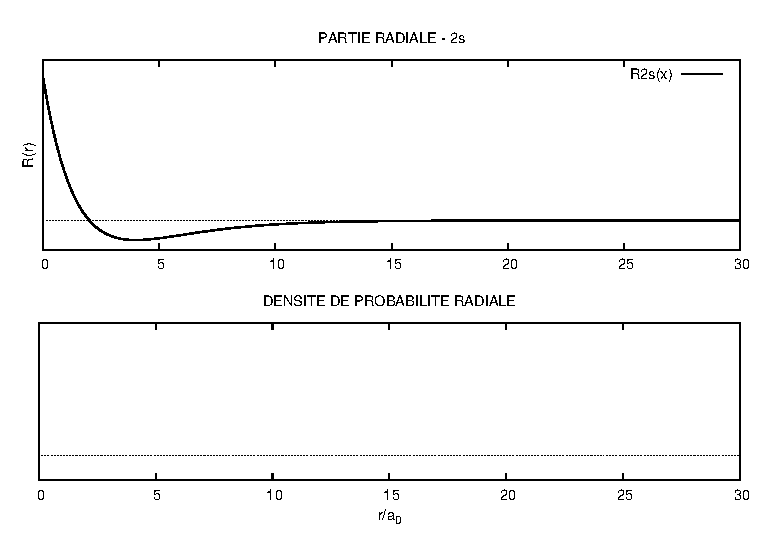
\includegraphics[angle=90,width=\textwidth]{figure/rad2s.eps}
\end{center}
\clearpage

\begin{center}
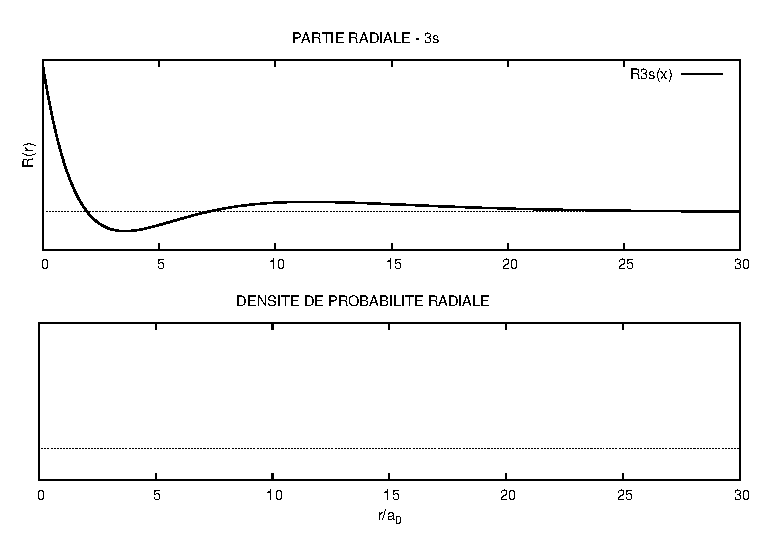
\includegraphics[angle=90,width=\textwidth]{figure/rad3s.eps}
\end{center}
\clearpage

\exo{Normation d'une fonction d'onde $-$ Repr\'esentation graphique}

L'\'etat fondamental de l'atome d'hydrog\`ene est d\'ecrit par la fonction d'onde~:

\[
%\Psi_{1s}(r,\theta,\varphi)=N.e^{-r/a_0} \qquad \textrm{avec~}N\textrm{~scalaire}
\begin{array}{rcl}
\Psi_{1s}(r,\theta,\varphi) &=& R(r) Y(\theta,\varphi) \qquad \text{o\`u}\\[0.3cm]
R(r)                        &=& N_r e^{-r/a_0}        \\
Y(\theta,\varphi)           &=& N_{\theta,\varphi} f(\theta,\varphi) \qquad f(\theta,\varphi) = 1\\
\end{array}
\]
avec $N_r$ et $N_{\theta,\varphi}$ scalaires.

\begin{enumerate}[\bf 1)]
\item Sachant qu'en coordonn\'ees sph\'eriques l'\'el\'ement diff\'erentiel de volume s'\'ecrit

$$
dV=d\tau=r^2\sin{\theta}dr d\theta d\varphi
$$

et que l'ensemble de l'espace est d\'ecrit lorsque $r$ varie de $0$ \`a $+\infty$, 
$\theta$ de $0$ \`a $\pi$ et $\varphi$ de $0$ \`a $2\pi$, \'ecrire l'expression de l'int\'egrale de 
normalisation.\\

\item \'Ecrire cette int\'egrale sous la forme d'un produit d'une int\'egrale angulaire~:
\[ 
N_{\theta,\varphi}^2 \int_0^\infty \int_0^{2\pi} f(\theta,\varphi) \sin{\theta} d\theta d\varphi
\]
et d'une int\'egrale radiale que vous det\'erminerez. Normer-les s\'eparemment.

\textbf{On donne~:} $\displaystyle \int_0^{+\infty}r^ne^{-Ar}dr=\frac{n!}{A^{n+1}}$ 
avec $n$, entier et $A$, r\'eel $> 0$.

\item \'Ecrire la $\Psi_{1s}(r,\theta,\varphi)$ totale. 

\item Rappeler les d\'efinitions de la probabilit\'e de pr\'esence et de la densit\'e 
de probabilit\'e radiale. Donner l'expression de la densit\'e de probabilit\'e radiale 
en fonction de la partie radiale $R_{n,l}$ d'une fonction d'onde.

\item Pour la fonction d'onde $\Psi_{1s}$, repr\'esenter graphiquement la courbe donnant, 
en fonction de $r/a_0$ dans l'intervalle $0 \leq r/a_0 \leq 5$, la densit\'e de 
probabilit\'e radiale.
\end{enumerate}


\exo{Repr\'esentation d'orbitale}
L'expression de l'orbitale $1s$ en un point $ M$ de coordonn\'ees  
$(r,\theta,\varphi)$ dans le cas de l'atome d'hydrog\`ene est donn\'ee par~:

$$
\Psi_{1s}(M)=N_s e^{-r/a_0} \ \text{,}
$$

et l'expression de l'orbitale $2p_z$~: 

$$
\Psi_{2p_z}(M)=
N_{p_z}\left(\frac{r}{a_0}\right)e^{-r/2a_0}\cos{\theta} \ .
$$

La densit\'e \'electronique est donn\'ee par~:
$$
D(M)=\Psi^\star(M)\Psi(M)=|\Psi(M)|^2  \ .
$$

\begin{enumerate}

\item Pour l'orbitale $2p_z$, donnez en fonction de $r/a_0$ l'expression de la 
densit\'e \'electronique pour l'ensemble des points $M$ situ\'es sur les axes $Ox$, $Oy$ et $Oz$.

\item Pour l'orbitale $2p_z$, donnez en fonction de $r/a_0$ l'expression de la 
densit\'e \'electronique pour l'ensemble des points $M$ situ\'es que sur l'axe $Oz$. 
Montrez que cette fonction $D(M)$ est maximale pour $r/a_0=2$ 
(tant vers les $z$ positifs, $\theta=0$, que vers les $z$ n\'egatifs, $\theta=180\deg$).

\item Pour quelle valeur de $\theta$ l'orbitale $2p_z$ vaut-elle z\'ero~? Quel est donc le plan nodal~?
Quelle est la densit\'e sur ce plan nodal~?

\item Pour l'orbitale $1s$, donnez en fonction de $r/a_0$ l'expression de la densit\'e 
\'electronique pour l'ensemble des points $M$ situ\'es sur les axes $Ox$, $Oy$ et $Oz$. 
Commentez.
\end{enumerate}

%Expression analytique des parties radiales~:
%
%\[
%\begin{array}{lll} 
%R_{1s}(r)  & = &  2 a_0^{-3/2} e^{-r/a_0}\\[0.3cm]
%R_{2s}(r)  & = &  \displaystyle{\frac{1}{\sqrt{2}} a_0^{-3/2} (1 - \frac{r}{2a_0}) e^{-r/2a_0}}\\[0.3cm]
%R_{3s}(r)  & = &  \displaystyle{\frac{2}{3\sqrt{3}} a_0^{-3/2} (1 - \frac{2r}{3a_0} + \frac{2r^2}{27a_0^2}) e^{-r/3a_0}}\\
%\end{array}
%\] 

\exo{R\'ecapitulatif sur les orbitales atomiques}
Soit un tableau relatif aux fonctions d'onde de l'atome d'hydrog\`ene.

\begin{center}
\begin{tabular}{|l|c|c|c|c|c| c|}\hline
orbitales & $R(r)$ & $Y(\theta,\varphi)$ & $E$ (eV) & $n$ & $l$ &  $m_l$\\\hline
$1s$   &           &                     & & & &\\\hline
$2s$   & \textbf{e}&                     & & & &\\\hline
$2p_x$ &           & \textbf{f}          & & & &\cellcolor{gray} \\\hline
$2p_y$ &           &                     & & & &\cellcolor{gray}\\\hline
$2p_z$ &           &                     & & & &\\\hline
\end{tabular}
\end{center}

On donne dans le d\'esordre les expressions des parties radiales et des parties angulaires norm\'ees s\'epar\'ement~:\\
$$
\textbf{a}=2\left(a_0^{-3/2}\right)e^{-r/a_0} \qquad \qquad
\textbf{b}=\frac{\sqrt{3}}{2\sqrt{\pi}}\sin{\theta}\sin{\varphi} \qquad \qquad
\textbf{c}=\frac{1}{2\sqrt{6}}\left(a_0^{-5/2}\right)r.e^{-r/2a_0}
$$
$$
\textbf{d}=\frac{1}{2\sqrt{\pi}}\qquad
\textbf{e}=\frac{1}{\sqrt{2}}\left(a_0^{-3/2}\right)\left(1-\frac{r}{2a_0}\right)e^{-r/2a_0}\qquad
\textbf{f}=\frac{\sqrt{3}}{2\sqrt{\pi}}\sin{\theta}\cos{\varphi}\qquad
\textbf{g}=\frac{\sqrt{3}}{2\sqrt{\pi}}\cos{\theta}
$$

\begin{enumerate}[\bf 1)]
\item Compl\'etez le tableau ci-dessus en pla\c{c}ant dans la case correspondant \`a chaque fonction d'onde, ($1s$, $2s$, $2p_x$, $2p_y$, $2p_z$) les lettres attribu\'ees aux fonctions radiales et angulaires convenables (\textbf{a}, \textbf{b}, \textbf{c}, \textbf{d}, \textbf{e}, \textbf{f} ou \textbf{g}, ci-dessus).\\

\textbf{Remarque~:} une m\^eme fonction peut intervenir dans diff\'erentes cases~: justifiez.

\item On donne les valeurs des \'energies de ces fonctions d'onde~: $-3,$4~eV et $-13,$6~eV. Placez ces valeurs dans les cases convenables du tableau. Pourquoi n'y a-t-il que deux valeurs~?

\item Compl\'etez le tableau en indiquant les valeurs des trois nombres quantiques orbitaux (ou nombres quantiques d'espace) pour chaque fonction d'onde.\\

\textbf{Remarque~:} pour les fonctions $2p_x$, $2p_y$, $2p_z$, justifiez la ou les valeurs de $m_l$ retenue(s) dans chaque cas.

\item Indiquez sch\'ematiquement les volumes de plus grande probabilit\'e de pr\'esence pour un \'electron $1s$, $2s$, $2p_x$, $2p_y$ ou $2p_z$, gravitant autour d'un noyau situ\'e au centre d'un rep\`ere orthonorm\'e.
\item Pr\'ecisez pour chaque orbitale :
\begin{enumerate}
\item le signe que prend la fonction d'onde dans les diff\'erentes r\'egions de l'espace~;
\item les surfaces nodales, le cas \'ech\'eant~;
\item les propri\'et\'es directionnelles et \'eventuellement les axes de r\'evolution.
\end{enumerate}
\end{enumerate}

